\section{Motor de búsquedas en el blockchain}
\label{sec:search}

\subsection{Introducción}

As an increasing number of smart contracts are deployed by developers, searching needs for massive smart contracts soar. Given that smart contracts are simply code and include no functional descriptions, indexing smart contracts with search engine technologies imposes a high difficulty. To index smart contracts properly, we use the following methods:

\begin{itemize}
	\item Crawl webpage data relevant to smart contracts to set up mappings between the data and blockchain smart contracts.

	\item Encourage developers to upload verified source code of smart contracts, analyze the functions and semantics of the code, create indexes for the source code, and provide the searching function for similar contracts. For smart contracts without source code, decompile them for their source code.

	\item Establish standards for smart contracts so that any contracts matching those standards can be retrieved and found by users. Also, encourage developers to provide informational descriptions of contracts during smart contract creation. \\

	\begin{figure}[ht]
  	\centering
  	\begin{minipage}{.4\linewidth}
	\begin{lstlisting}[frame=single]
contract SearchableContract {
   string public language;
   string public author;
   string public name;
   string public title;
   string public description;
   string public tags;
}
	\end{lstlisting}
  	\end{minipage}
	\end{figure}

\end{itemize}

\subsection{Infrastructure}

In current stage, We think that the centralized search engine is more suitable for obtaining the best user experience and presenting the value of Nebulas Rank. The Nebulas development team is dedicated to developing a searching service, retrieving all smart contracts in real time, performing multilingual word breaking and creating full-text indexes to provide users with a user-friendly web interface. The impartiality of the NR ranking algorithm and the verifiability of each node ensure the impartiality of the centralized searching service, while the complete code of the searching backend is available to the community. Also, third-party developers can create their own searching services on this basis. \reffig{fig:search-arch} shows the architecture of the searching service.

\begin{figure}[h]
\centering
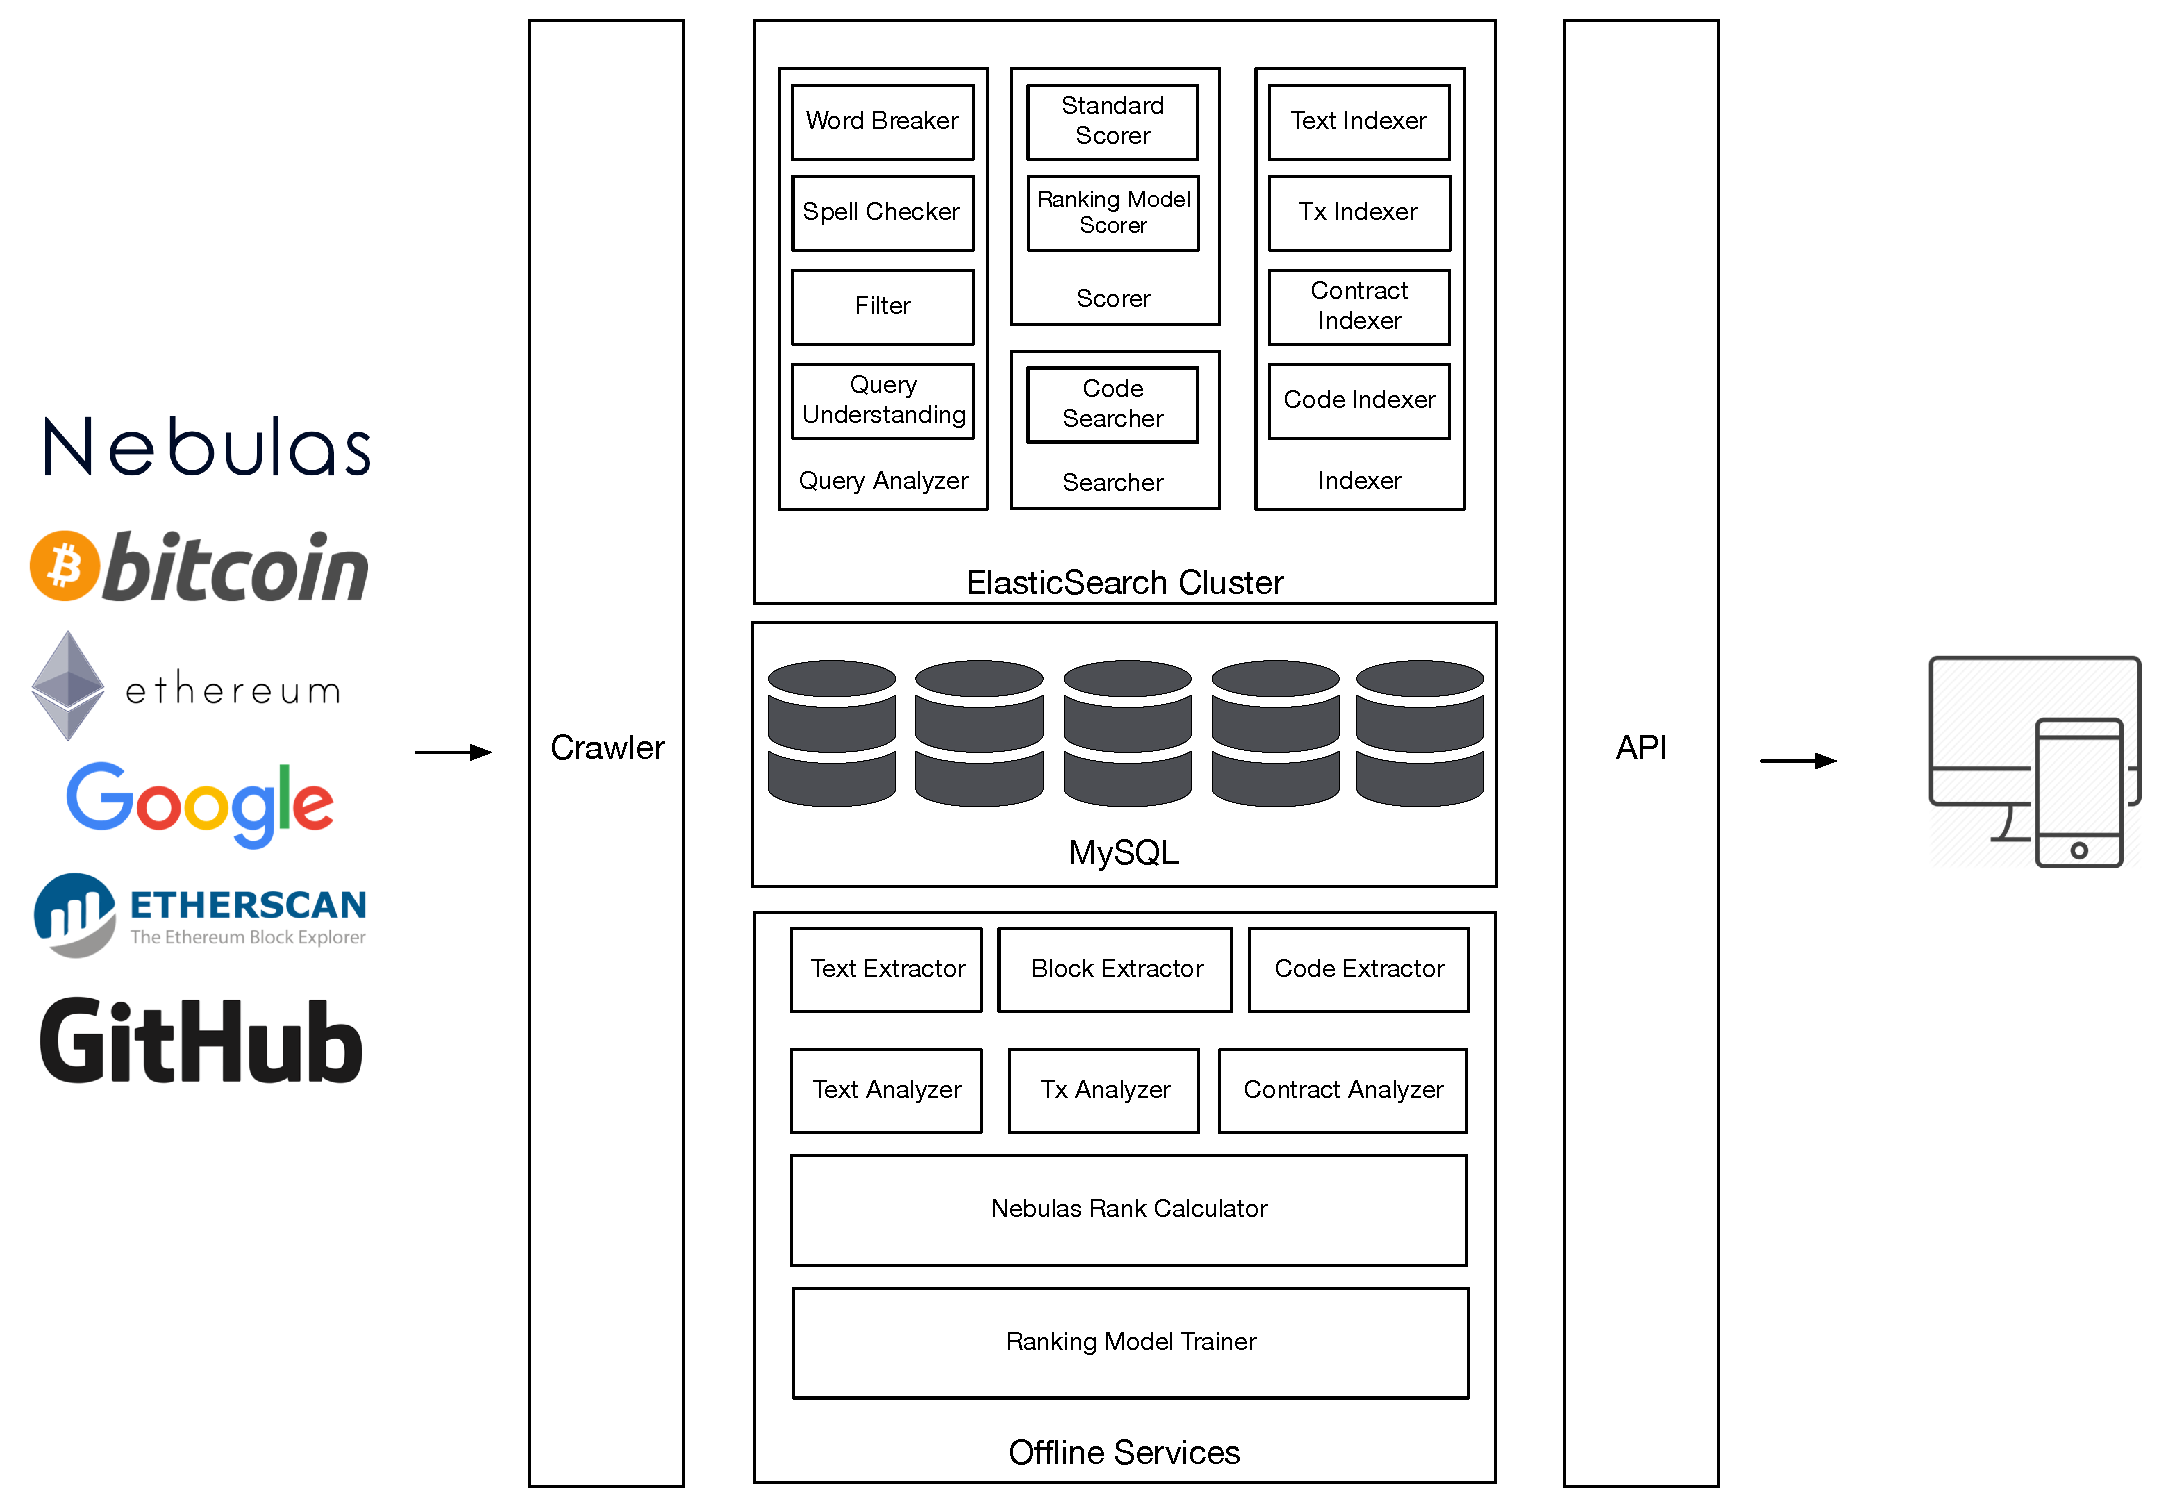
\includegraphics[width=16cm]{./figs/search-arch-new}
\caption{Architecture of the searching service}
\label{fig:search-arch}
\end{figure}

\begin{itemize}
	\item \textbf{Crawler}  data sources of the Crawler in blockchain search engine are classified into two types: one for collecting block information and code of smart contracts from blockchains, while the other for crawling data about smart contracts from public URLs including introductions, Dapp user comments and news.

	\item \textbf{Extractor} consists of Text Extractor, Block Extractor and Code Extractor, which provide text information, block information and code extraction service for smart contracts, respectively.

	\item \textbf{Analyzer} consists of Text Analyzer, Tx Analyzer and Contract Analyzer, which are text information, block transaction information and smart contract analyzers, respectively. For the smart contract analyzer, it provides contract decompilation, source code extraction, semantic analysis and so on.

	\item \textbf{Nebulas Rank Calculator} refers to the Nebulas Rank calculator service, which is used to calculate the Nebulas Ranks of each non-contract and contract accounts offline.

	\item \textbf{Ranking Model Trainer} refers to the ranking model trainer service. Ranking rules take multiple factors into account: matching field, text relevance, NR Rank value of the contract, transaction quantity of the contract, frequency and depth, NR Rank of the user conducting a transaction with the contract, and contract security. Based on users' actual use conditions, the machine learning algorithm (GBDT and artificial neural network (ANN) are optional) is used to train the ranking and scoring model, which is also constantly improved according to user feedback. The trained model is used by Scorer of the searching service.

	\item \textbf{Query Analyzer} refers to the keyword analysis service, which includes the multilingual word breaker (Word Breaker) and the spell checker (Spell Checker).

	\item \textbf{Indexer} creates proper indexes from Analyzer and supports both full and incremental indexing.

	\item \textbf{Scorer} is classified into two levels: Level-1 Standard Scorer recalls candidate result sets from ElasticSearch, which is done to recall as many candidate results as possible through the efficient and effective ranking in the ElasticSearch cluster. Level-1 can recall several thousands of results. Level-2 Ranking Model Scorer uses the offline rank model to calculate and reorder the rank of each Level-1 candidate result set. For this level, the calculated results feature a sounding accuracy and can be used directly by users.

	\item \textbf{Searcher} is responsible for communicating with the ElasticSearch cluster and packing and returning the search result to the searching frontend.

	\item \textbf{API} provides external applications with comprehensive searching API services.

	\item \textbf{ElasticSearch Cluster} ES refers to the server cluster. The Nebulas development team plans to use the open-source search engine ElasticSearch to support full-text indexing.

\end{itemize}

\subsection{Nebulas Trends}

The Nebulas creates the tendency list in combination with Nebulas Rank to provide user visual multi-dimensional values in blockchains.

\begin{itemize}
\item \textbf{Nebulas Rank list for non-contract accounts.} It displays the daily NR list and the NR quick rise and drop lists. Also, this rank list visualizes the rank variation tendency of each account and the health change tendency of the entire network.

\item \textbf{Nebulas Rank list for contract accounts.} Based on the NR values of non-contract accounts, the Nebulas Rank list calculates the NR list of contract accounts, the quick rise and drop lists, the variation tendency of each contract and the tendency chart for the quantity and use frequency of smart contracts on the entire network. In addition, we will present other smart contract lists such as the token contract list and the market contract estimation list to display a wider dimension of information.

\item \textbf{Smart contract developer list.} According to the contract account list, the list of smart contract developers calculates the contribution list of contract developers and the contribution quick rise list to display outstanding contracts developers and Dapps.

\end{itemize}

\subsection{Keyword Query}

By providing a keyword or describing the textual information about a smart contract such as its title, author or function, users can find the matching contract from massive smart contracts. Currently, mature and sophisticated algorithms and technologies are available for text searching. By using the natural language processing and inverted index technologies, we can retrieve and sort efficiently in the index database for massive smart contracts. This involves the following key technologies:

\begin{enumerate}
	\item Topic-oriented distributed crawler technology
	\item Multilingual word breaking technology: word breaking is relatively simple for western words. For the word breaking of Chinese words, these algorithms are available: positive maximum matching, negative maximum matching, shortest path word breaking and statistical word breaking.
	\item Search term correction and semantic comprehension
	\item Inverted index and distributed searching architecture
	\item Ranking algorithm to sort the search results

\end{enumerate}

Among these technologies, the ranking algorithm will be designed in combination with Nebulas Rank. Specifically, we use intra-user transfers in the blockchain world as an analogy to webpage reference relations in the Internet world to create the blockchain transaction graph. Then, calculate the NR rank of non-contract accounts by using the NR ranking algorithm described in Section 2.3, calculate the ranks of those contracts by using the contract ranking algorithm described in Section 4.2, and lastly use the calculation result for search result sorting.


\subsection{Searching for Similar Smart Contracts}

For developers and certain users, they may want to search for smart contracts with similar functions according to the code fragment of a contract. Being different from regular keyword searching, code similarity has its particularity. To implement the searching function for similar smart contracts, we need to use a certain algorithm to measure the code similarity in a number or percentage.

In today's academia, code similarity algorithms are mainly categorized into the string edit distance, token sequence similarity, abstract syntax tree similarity and program dependency graph similarity. These algorithms describe the similarity in terms of code text, structure and syntax from different dimensions. By combining these 4 major algorithms, we put forward 12 features of the code similarity of Nebulas contracts, such as Skeleton Tree, Type Signature and Library Calls. For details, see Appendix \ref{appendix:sim_code}.

Similar to search results of keywords, search results of smart contracts also use the same contract ranking algorithm to sort final results.